%% ASP-DAC 2027 camera-ready. ACM sigconf (sample-sigconf).
%% Compile: latexmk (pdflatex x2 + bibtex). acmart provides amsmath/graphicx/hyperref/xcolor/url.
\documentclass[sigconf]{acmart}
\makeatletter
\AtBeginDocument{\global\@ACM@balancefalse}
\makeatother

% TODO(camera-ready): replace with the exact rights text, DOI and ISBN from the ACM rights form.
\setcopyright{acmlicensed}
\copyrightyear{2027}
\acmYear{2027}
\acmDOI{XXXXXXX.XXXXXXX}
\acmConference[ASPDAC '27]{32nd Asia and South Pacific Design Automation Conference}{January 25--28, 2027}{Tokyo, Japan}
\acmBooktitle{32nd Asia and South Pacific Design Automation Conference (ASPDAC '27), January 25--28, 2027, Tokyo, Japan}
\acmISBN{978-x-xxxx-xxxx-x/YYYY/MM}

\usepackage{booktabs}
\usepackage{float}
\usepackage{algorithm}
\usepackage[noend]{algpseudocode}
\usepackage{tikz}
\usetikzlibrary{arrows.meta,positioning,calc,backgrounds,decorations.pathreplacing}


\newcommand{\mmapopc}{\texttt{and.popc}}

\begin{document}

\title{TensorLUT: Exact Batched RTL Simulation via ANF-Lifted Tensor-Core GEMM}

\author{Zhengyi Zhang}
\email{zhengyizhang24@m.fudan.edu.cn}
\affiliation{%
  \department{State Key Laboratory of Integrated Chips and Systems}
  \institution{Fudan University}
  \city{Shanghai}
  \country{China}}

\author{Sijing Yang}
\email{sjyang24@m.fudan.edu.cn}
\affiliation{%
  \department{State Key Laboratory of Integrated Chips and Systems}
  \institution{Fudan University}
  \city{Shanghai}
  \country{China}}

\author{Yuwei Qu}
\email{ywqu24@m.fudan.edu.cn}
\affiliation{%
  \department{State Key Laboratory of Integrated Chips and Systems}
  \institution{Fudan University}
  \city{Shanghai}
  \country{China}}

\author{Zixuan Xiao}
\email{22307130371@m.fudan.edu.cn}
\affiliation{%
  \department{State Key Laboratory of Integrated Chips and Systems}
  \institution{Fudan University}
  \city{Shanghai}
  \country{China}}

\author{Lingli Wang}
\authornote{Corresponding author.}
\email{llwang@fudan.edu.cn}
\affiliation{%
  \department{State Key Laboratory of Integrated Chips and Systems}
  \institution{Fudan University}
  \city{Shanghai}
  \country{China}}

\renewcommand{\shortauthors}{Z. Zhang et al.}

\begin{abstract}
Regression verification runs one compiled design against thousands of independent seeds. TensorLUT
makes those seeds the rows of a matrix product and runs exact 2-state, single-clock LUT/DFF
simulation on NVIDIA tensor cores. The mapping rests on two facts: an AND of $k$ bits is true exactly
when their popcount is $k$, and an XOR is a parity. Written in algebraic normal form (ANF), each LUT
layer becomes two single-bit \mmapopc{} matrix products, the first followed by a degree check and the
second by a parity. A tensor-core-aware compiler sends affine cones to one GF(2) GEMM, lowers bounded
nonlinear cones to term-reduced ESOP, and tiles wide cones as levelized LUT-ANF. Every route keeps
the synthesized LUT semantics, and traces match Icarus Verilog bit for bit at each cycle boundary. On
one RTX~4090, TensorLUT reaches $3.0\times10^9$ cycle$\cdot$stimuli/s on algebraic microbenchmarks.
On RTeAAL's RocketChip core it sustains $9.5\times10^6$, $7.0\times$ the throughput of 80 Verilator
processes on a 40-core server and $242\times$ that of one, and scales to $4.0\times10^7$ on four GPUs.
Against RTLflow, a published GPU simulator, it is up to $2.5\times$ faster for batches up to $2^{12}$
seeds and reaches 80\% of RTLflow's throughput at larger batches, while compiling $65\times$ faster.
\end{abstract}

\ccsdesc[500]{Hardware~Simulation and emulation}
\ccsdesc[500]{Hardware~Hardware accelerators}
\ccsdesc[300]{Computing methodologies~Parallel computing methodologies}

\keywords{RTL simulation, cycle-accurate, tensor cores, GF(2), ANF, ESOP synthesis, GPU}

\maketitle

\section{Introduction}
RTL simulation serves two different goals. A directed test needs low latency for one run; a
regression needs high throughput across many seeds. Constrained-random verification runs $10^4$ to
$10^5$ seeds against the same netlist~\cite{crv}, and coverage-directed fuzzing~\cite{rfuzz} and fault
simulation~\cite{ppsfp} also run one fixed design against many independent stimuli. These stimuli
form a batch that a GPU can simulate in parallel. This paper targets simulation throughput for such
batches; we do not build a fuzzer or a fault simulator on top of it.

GPU RTL simulators already exist, but none of them puts the Boolean update on tensor cores. RTLflow
transpiles Verilator's schedule to CUDA kernels that run many stimuli at once~\cite{rtlflow}, and GEM
emulates an FPGA-like Boolean processor on CUDA cores~\cite{gem}. On the CPU side, RTeAAL~Sim casts
RTL simulation as sparse tensor algebra~\cite{rteaal} and GSIM generates faster simulators~\cite{gsim}.
These simulators evaluate one gate or instruction at a time, with irregular fan-in,
data-dependent indexing, and AND/XOR operators that a numeric MMA unit does not provide. Tensor cores
instead execute dense, regular matrix products. Tensor-core sparse kernels such as TC-GNN~\cite{tcgnn} and DTC-SpMM~\cite{dtcspmm} show how to
tile irregular matrices for these units, but they compute numeric kernels, not clocked state updates.

TensorLUT obtains such matrix products from two observations. First, independent seeds form the rows
of a matrix: every seed runs the same netlist, so a batch turns each logic layer into a tall matrix
product. Second, a LUT
layer already has an algebraic form that tensor cores can evaluate. In ANF each output is an XOR of AND
monomials, and a monomial such as $x_i x_j$ is true exactly when the number of its asserted inputs
equals its size, its \emph{degree}. A popcount gives that number. One \mmapopc{} product against a
monomial-incidence matrix therefore builds every AND term at once, a degree check keeps the true ones,
and a second \mmapopc{} product followed by a parity combines them into each LUT output. Throughout,
\emph{exact} means bit-exact under 2-state, single-clock, cycle-boundary semantics;
Sec.~\ref{sec:scope} discusses X/Z values, multiple clocks, and memories.

\textbf{Key idea.} A clock edge over a 2-state LUT/DFF netlist is a sequence of layers, and each
layer is \emph{Boolean feature construction} followed by a \emph{GF(2) linear combination}. Both steps
are matrix products that tensor cores can execute, and together they compute the same outputs as
the LUT network. For a layer with
input signals $X$ (batch $\times$ inputs), monomial-incidence matrix $A$, per-monomial
degrees $s$, and ANF coefficient matrix $C$:
\begin{equation}
Y \;=\; \bigl(\mathbf{1}[\,X A = s\,]\bigr)\, C \pmod 2 .
\label{eq:anf}
\end{equation}
Here $\mathbf{1}[XA=s]$ builds the AND-monomial features, since a monomial is true when its
asserted support count equals its degree. The second product and the parity compute each LUT
output's XOR. Both products use single-bit \mmapopc{}; the compare and the parity are short
epilogues.

Fig.~\ref{fig:flow} shows the compiler. It extracts next-state cones, strips constants and copies,
routes affine cones to one GF(2) GEMM, and routes bounded nonlinear cones to a term-reduced ESOP
plan. When that whole-cone ESOP is too wide, the compiler returns to the LUT levels and chunks each
layer's monomial dimension into tensor-core-sized blocks. The design-dependent tensors ($A$, $s$,
and $C$) are compiled once and kept resident; runs stream only stimuli and sampled outputs.

\begin{figure*}[t]
\centering
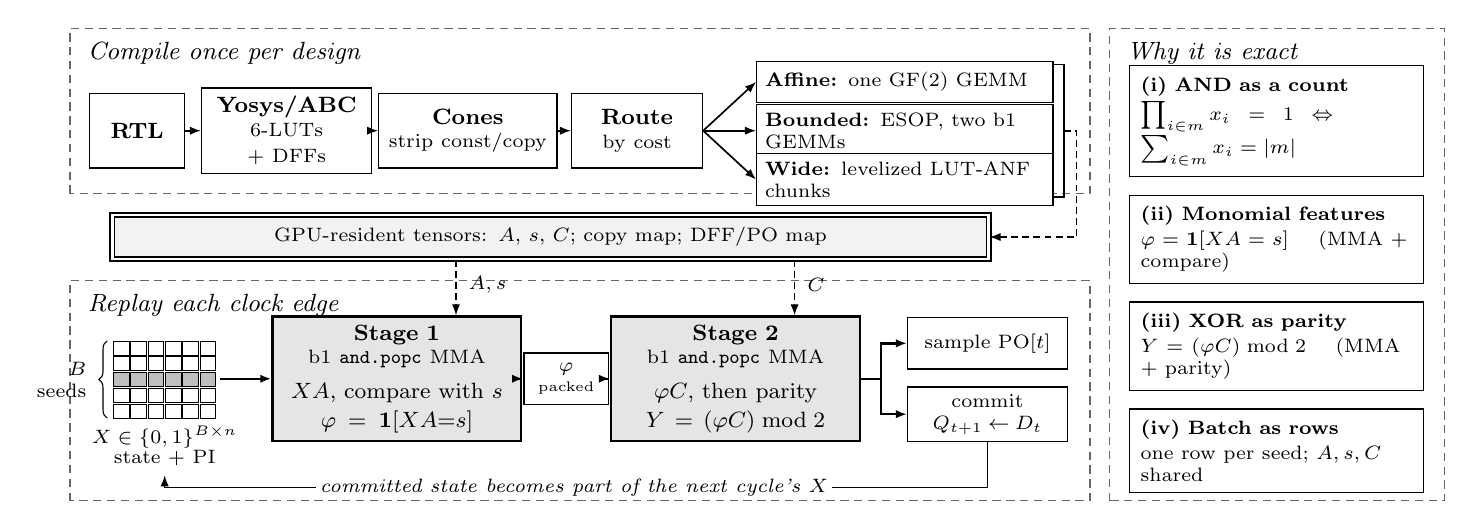
\begin{tikzpicture}[
  font=\footnotesize,
  >={Latex[length=4pt,width=3pt]},
  step/.style={draw=black,line width=0.5pt,fill=white,align=center,inner sep=3pt,
               minimum height=9.5mm,text width=#1},
  plan/.style={draw=black,line width=0.5pt,fill=white,align=left,inner sep=3pt,
               minimum height=5.2mm,text width=3.55cm,font=\scriptsize},
  stage/.style={draw=black,line width=0.8pt,fill=black!10,align=center,inner sep=3pt,
                minimum height=15.5mm,text width=2.95cm},
  small/.style={draw=black,line width=0.5pt,fill=white,align=center,inner sep=2.5pt,
                minimum height=6.5mm,font=\scriptsize},
  law/.style={draw=black,line width=0.4pt,fill=white,align=left,inner sep=4pt,
              text width=3.45cm,font=\scriptsize,minimum height=10.5mm},
  frame/.style={draw=black!60,line width=0.5pt,dash pattern=on 3pt off 2pt},
  arr/.style={->,line width=0.6pt},
  data/.style={->,line width=0.6pt,dash pattern=on 2.5pt off 1.5pt},
  flow/.style={->,line width=0.9pt},
  sub/.style={font=\scriptsize},
]
% ---- group frames ----
\draw[frame] (0,4.2) rectangle (12.95,6.3);
\draw[frame] (0,0.3) rectangle (12.95,3.1);
\draw[frame] (13.2,0.3) rectangle (17.45,6.3);
\node[anchor=north west,font=\small\itshape] at (0.1,6.25) {Compile once per design};
\node[anchor=north west,font=\small\itshape] at (0.1,3.05) {Replay each clock edge};
\node[anchor=north west,font=\small\itshape] at (13.3,6.25) {Why it is exact};

% ---- compile flow ----
\node[step=1.0cm] (RTL) at (0.85,5.0) {\textbf{RTL}};
\node[step=1.95cm] (YS) at (2.75,5.0) {\textbf{Yosys/ABC}\\[-1pt]{\scriptsize 6-LUTs + DFFs}};
\node[step=2.05cm] (CN) at (5.05,5.0) {\textbf{Cones}\\[-1pt]{\scriptsize strip const/copy}};
\node[step=1.45cm] (RT) at (7.2,5.0) {\textbf{Route}\\[-1pt]{\scriptsize by cost}};
\node[plan] (P1) at (10.6,5.62) {\textbf{Affine:} one GF(2) GEMM};
\node[plan] (P2) at (10.6,5.0) {\textbf{Bounded:} ESOP, two b1 GEMMs};
\node[plan] (P3) at (10.6,4.38) {\textbf{Wide:} levelized LUT-ANF chunks};
\draw[arr] (RTL) -- (YS);
\draw[arr] (YS) -- (CN);
\draw[arr] (CN) -- (RT);
\foreach \p in {P1,P2,P3} \draw[arr] (RT.east) -- (\p.west);

% ---- GPU-resident tensors ----
\node[draw=black,line width=0.5pt,double,double distance=1pt,fill=black!5,minimum height=5.6mm,
      text width=10.9cm,align=center,font=\scriptsize] (STORE) at (6.1,3.65)
  {GPU-resident tensors: $A$, $s$, $C$; copy map; DFF/PO map};
\draw[line width=0.5pt] (12.5,5.84) -- (12.62,5.84) -- (12.62,4.16) -- (12.5,4.16);
\draw[data] (12.62,5.0) -- (12.78,5.0) |- (STORE.east);

% ---- replay ----
\foreach \r in {0,...,4} \foreach \c in {0,...,5}
  \draw[black,line width=0.3pt,fill=white] (0.55+0.22*\c,1.35+0.2*\r) rectangle +(0.2,0.18);
\foreach \c in {0,...,5}
  \draw[black,line width=0.3pt,fill=black!25] (0.55+0.22*\c,1.75) rectangle +(0.2,0.18);
\draw[decorate,decoration={brace,amplitude=3pt,mirror},line width=0.4pt]
  (0.47,2.33) -- (0.47,1.35) node[midway,left=4pt,sub,align=right]{$B$\\seeds};
\node[sub,align=center] (X) at (1.2,1.0) {$X\in\{0,1\}^{B\times n}$\\[-1pt]state + PI};
\node[stage] (S1) at (4.15,1.85)
  {\textbf{Stage 1}\\[-1pt]{\scriptsize b1 \mmapopc{} MMA}\\[3pt]
   $XA$, compare with $s$\\[1pt]$\varphi=\mathbf{1}[XA{=}s]$};
\node[small,text width=0.9cm] (PHI) at (6.3,1.85) {$\varphi$\\[-1pt]{\tiny packed}};
\node[stage] (S2) at (8.45,1.85)
  {\textbf{Stage 2}\\[-1pt]{\scriptsize b1 \mmapopc{} MMA}\\[3pt]
   $\varphi C$, then parity\\[1pt]$Y=(\varphi C)\bmod 2$};
\node[small,text width=1.85cm] (PO) at (11.65,2.3) {sample PO$[t]$};
\node[small,text width=1.85cm] (CE) at (11.65,1.4) {commit $Q_{t+1}\!\leftarrow\!D_t$};
\draw[flow] (1.9,1.85) -- (S1.west);
\draw[flow] (S1.east) -- (PHI.west);
\draw[flow] (PHI.east) -- (S2.west);
\coordinate (split) at (10.3,1.85);
\draw[flow,-] (S2.east) -- (split);
\draw[flow] (split) |- (PO.west);
\draw[flow] (split) |- (CE.west);
\draw[data] ($(STORE.south -| S1.north)+(0.75,0)$) -- ($(S1.north)+(0.75,0)$) node[pos=0.45,right=1pt,font=\scriptsize]{$A,s$};
\draw[data] ($(STORE.south -| S2.north)+(0.75,0)$) -- ($(S2.north)+(0.75,0)$) node[pos=0.45,right=1pt,font=\scriptsize]{$C$};
\draw[arr] (CE.south) -- (11.65,0.47) -- (1.2,0.47) -- (X.south);
\node[font=\scriptsize\itshape,fill=white,inner sep=1.5pt] at (6.4,0.47)
  {committed state becomes part of the next cycle's $X$};

% ---- why it is exact ----
\node[law] (L1) at (15.32,5.12) {\textbf{(i) AND as a count}\\[1pt]
  $\prod_{i\in m}x_i=1 \Leftrightarrow \sum_{i\in m}x_i=|m|$};
\node[law,below=2.2mm of L1] (L2) {\textbf{(ii) Monomial features}\\[1pt]
  $\varphi=\mathbf{1}[XA=s]$ \quad (MMA + compare)};
\node[law,below=2.2mm of L2] (L3) {\textbf{(iii) XOR as parity}\\[1pt]
  $Y=(\varphi C)\bmod 2$ \quad (MMA + parity)};
\node[law,below=2.2mm of L3] (L4) {\textbf{(iv) Batch as rows}\\[1pt]
  one row per seed; $A,s,C$ shared};
\end{tikzpicture}
\caption{TensorLUT's lowering and replay path. The compiler reduces RTL to LUT/DFF cones and emits
one of three tensor-core execution plans: affine GF(2) GEMM, bounded ESOP, or levelized LUT-ANF
chunks. The resulting tensors $A,s,C$ and signal maps remain resident on the GPU. At each clock edge,
a batch $X$ flows through two single-bit tensor-core products: Stage~1 builds
$\varphi=\mathbf{1}[XA{=}s]$ and Stage~2 computes $Y=(\varphi C)\bmod 2$ before sampling outputs
and committing state.}
\Description{A restrained schematic with two horizontal lanes and a formula sidebar. The top lane
shows compile-time lowering from RTL through Yosys/ABC, cone extraction, routing, and three plan
choices. A device-resident artifact containing A, s, C, and signal maps feeds the lower runtime lane.
The runtime lane maps a batch of seeds to rows of X, runs two b1 tensor-core matrix products, samples
primary outputs, and feeds committed state back into the next cycle. The sidebar lists the monomial
count identity, feature construction, ANF parity, and batch-row mapping.}
\label{fig:flow}
\end{figure*}

\textbf{Contributions.}
\begin{enumerate}
\item An \emph{ANF-lifted GEMM} formulation for 2-state LUT evaluation, with a proof
and a worked example (Sec.~\ref{sec:form}).
\item A compiler that maps affine cones to one GF(2) matrix, lowers bounded cones to
term-reduced ESOP, and repairs wide cones with levelized LUT-ANF tiling (Sec.~\ref{sec:compiler}).
\item A GPU backend that keeps the matrices resident, bit-packs features, and runs both stages on
binary tensor cores (Sec.~\ref{sec:backend}).
\item An evaluation on an RTX~4090 (Sec.~\ref{sec:eval}): Icarus Verilog differentials, batch
sweeps from 1 to $2^{19}$ seeds against measured multi-process Verilator, a CUDA-core baseline, and
the published GPU simulators RTLflow and GEM, a compile-time breakdown, LUT-width and ESOP ablations,
and multi-GPU scaling on RocketChip.
\end{enumerate}

\section{Background}
\textbf{LUT/DFF netlists.} We target single-clock, edge-triggered, 2-state designs after frontend
normalization. Yosys~\cite{yosys} lowers RTL to $k$-input LUTs (\texttt{abc -lut}) and positive-edge D
flip-flops; reset/enable, including the asynchronous resets in ISCAS'89, fold into combinational
next-state logic under the cycle-boundary 2-state semantics we check.
The cone feeding each register/output is levelized into topological \emph{layers}; a clock edge
evaluates all layers then commits each flop's D to Q.

\textbf{Algebraic Normal Form.} Every Boolean function has a unique ANF (Zhegalkin polynomial)
$f(x)=\bigoplus_{m\in M}\prod_{i\in m} x_i$. XOR/NOT are degree $\le 1$; each AND raises degree.
Because we simulate one edge at a time, only the \emph{per-layer} degree matters, bounded by the
LUT width $k$ ($\le 6$).

\textbf{Single-bit tensor cores.} NVIDIA tensor cores expose a 1-bit (\texttt{b1}) operation that
ANDs 1-bit operands and accumulates their popcount into int32 (\texttt{mma\dots b1.\mmapopc}). The
two ANF stages use that count directly. A 1-bit contraction tile holds 128 elements in a 32-bit
word, which suits the wide sparse monomial supports of a LUT layer, and the popcount is the integer
count used by Eqs.~\eqref{eq:count} and~\eqref{eq:parity}.

\textbf{Batched simulation as a cost model.} With a fixed design and $B$ independent stimuli, each
cycle evaluates the same layered circuit $B$ times. A CPU simulator reuses compiled code but still
runs seeds one after another on each core. TensorLUT puts seeds on the matrix row dimension, so a
layer becomes a tall GEMM and arithmetic intensity rises with $B$. The relevant metric is
throughput, not single-seed latency.

\section{ANF-Lifted GEMM}\label{sec:form}
\subsection{Layer Equations and Exactness}
Let a layer have $n$ inputs, $F$ distinct monomials, $G$ LUT outputs, and encode $B$ stimuli as
$X\in\{0,1\}^{B\times n}$. Define incidence $A\in\{0,1\}^{n\times F}$ ($A_{i,f}=1$ iff input $i$
is in monomial $f$), degrees $s_f=\sum_i A_{i,f}$, and coefficients $C\in\{0,1\}^{F\times G}$
($C_{f,g}=1$ iff monomial $f$ appears in output $g$'s ANF).

\textbf{Lemma 1 (LUT$\rightarrow$ANF).} Every Boolean $f:\{0,1\}^k\!\to\!\{0,1\}$ has a unique
ANF, obtained from its truth table by the M\"obius transform in $O(k\,2^k)$; constant inputs are
folded by restricting the truth table before the transform.

\textbf{Lemma 2 (monomial as count).} For $x\in\{0,1\}$ and a monomial $m$,
\begin{equation}
\prod_{i\in m} x_i = 1 \;\Longleftrightarrow\; \sum_{i\in m} x_i = |m| .
\label{eq:count}
\end{equation}
Thus the feature matrix $\varphi=\mathbf{1}[\,XA=s\,]$ gives, per stimulus and monomial, the exact
AND-monomial value: $XA$ is an integer matrix product ($X\!\in\!\{0,1\}^{B\times n}$,
$A\!\in\!\{0,1\}^{n\times F}$) that counts, for each stimulus, how many of a monomial's support
inputs are set, and the elementwise test against the degree $s$ decides the monomial.

\textbf{Lemma 3 (XOR as parity).} Since ANF combines monomials by XOR,
\begin{equation}
y_g \;=\; \bigoplus_{f} C_{f,g}\,\varphi_f \;=\; \Bigl(\textstyle\sum_{f} C_{f,g}\,\varphi_f\Bigr)
\bmod 2 ,
\label{eq:parity}
\end{equation}
so $Y=(\varphi C)\bmod 2$: $\varphi C$ is an integer matrix product and $\bmod\,2$ is a
bitwise-and-one epilogue.

\textbf{Theorem.} Combining Lemmas~1--3, Eq.~\eqref{eq:anf} equals the exact 2-state LUT-layer
outputs for all stimuli. Evaluating layers in topological order within a cycle and committing
each flip-flop's $D$ to $Q$ at the edge reproduces the reference cycle-accurate trace
bit-for-bit. The two integer products carry counts bounded by $n$ (resp.\ $F$), well within
int32; encoding the $\{0,1\}$ operands as single bits, both products are realized by the
\texttt{b1 \mmapopc} tensor-core instruction, so the entire layer evaluation runs on tensor
cores except the (cheap) compare and parity.

\textbf{Affine as a degenerate case.} If every monomial is a singleton ($\deg\le 1$), stage~1 is
the identity ($\varphi=X$) and Eq.~\eqref{eq:anf} collapses to a \emph{single} GF(2) GEMM
$Y=(XC)\bmod2$. Composing such degree-1 cones along the DAG yields one transition matrix per
design; a clock edge becomes one \texttt{b1} GEMM with no AND-monomial stage.

\subsection{Example and Matrix Construction}
Consider a layer with inputs $(x_1,x_2,x_3)$ and two LUT outputs
\begin{equation}
y_1 = x_1 \oplus x_2 \oplus x_1 x_3, \qquad
y_2 = x_1 x_2 \oplus x_3 .
\label{eq:ex}
\end{equation}
Their ANFs use $F{=}5$ \emph{distinct} monomials, shared across the two outputs:
$m_1{=}x_1,\ m_2{=}x_2,\ m_3{=}x_3,\ m_4{=}x_1x_3,\ m_5{=}x_1x_2$, with degrees
$s=[\,1,1,1,2,2\,]$. The incidence and coefficient matrices are
\begin{equation}
A=\begin{bmatrix}
1&0&0&1&1\\
0&1&0&0&1\\
0&0&1&1&0
\end{bmatrix},
\qquad
C=\begin{bmatrix}
1&0\\
1&0\\
0&1\\
1&0\\
0&1
\end{bmatrix},
\label{eq:exAC}
\end{equation}
where column $f$ of $A$ is monomial $m_f$'s support over $(x_1,x_2,x_3)$ and column $g$ of $C$
marks the monomials in output $y_g$.

Take one stimulus $X=[\,1,1,0\,]$. Stage~1 forms the integer products and thresholds against the
degrees:
\begin{equation}
XA=[\,1,1,0,1,2\,],\quad
\varphi=\mathbf{1}[\,XA=s\,]=[\,1,1,0,0,1\,].
\label{eq:exphi}
\end{equation}
Reading $\varphi$: $m_1{=}x_1{=}1$, $m_2{=}x_2{=}1$ and $m_5{=}x_1x_2{=}1$ hold; $m_3{=}x_3{=}0$
and $m_4{=}x_1x_3{=}0$ do not---exactly $\mathrm{popc}(X\wedge A_{:,f})=s_f$, the \mmapopc{}
test. Stage~2 combines by parity:
\begin{equation}
\varphi C=[\,2,1\,],\quad
Y=(\varphi C)\bmod 2=[\,0,1\,],
\label{eq:exY}
\end{equation}
matching $y_1=1{\oplus}1{\oplus}0=0$ and $y_2=1{\oplus}0=1$ from Eq.~\eqref{eq:ex}. The same $A$,
$s$, $C$ drive all $B$ stimuli at once by stacking them as rows of $X$.

\textbf{Layer matrix construction.} The compiler builds the matrices of Eq.~\eqref{eq:anf} from a
levelized LUT/DFF netlist. For each layer it enumerates the layer-local input signals, applies the
M\"obius transform to every LUT truth table, interns each nonzero monomial support in a hash table,
and emits the bit-incidence matrix $A$, the degree vector $s$, and the sparse coefficient matrix
$C$. A constant term is a degree-0 monomial with an empty support column, so Eq.~\eqref{eq:count}
still holds with both the popcount and the threshold equal to zero. Working per layer keeps the
support bounded: a global ANF over an entire cone can grow with its transitive fan-in, whereas a
layer produced by \texttt{abc -lut 6} depends only on a handful of local signals. Interning is
shared within the layer, so a product such as $x_i x_j$ that appears in many LUTs is built once and
referenced by several columns of $C$.

\textbf{Integer counts, Boolean results.} The tensor core only accumulates popcounts. The Boolean
meaning comes from the epilogues. Stage~1 checks whether the support count equals the degree;
stage~2 takes parity. No stage treats a count as a real-valued activation or uses integer addition
as the circuit operation.

\section{Tensor-Core-Aware Synthesis}\label{sec:compiler}
The direct pipeline maps the design to $k$-LUTs, reads off each LUT's ANF, and unions the
monomials of a level. That gives an exact plan, but it optimizes a LUT mapper's objective: area,
depth, and LUT count. The cost of the tensor-core backend depends on other quantities.

\subsection{Cost Model and ESOP Lowering}
A monomial's degree is only the column weight of $A$, so a degree-6 monomial and a degree-2 monomial
use the same \texttt{b1} contraction tile. The expensive quantities are the number of distinct
monomials $F$, which sets the GEMM width, and the number of layers, since every layer adds two
GEMMs, a synchronization, and intermediate net-state traffic. The compiler targets those two
costs: fewer terms and fewer layers.

ESOP gives that representation: one XOR of arbitrary-polarity product terms over the whole
next-state cone. We run heuristic ESOP minimization~\cite{exorcism} on the cone's AIG. If the term
count fits the tensor-core budget, this produces one tensor-core layer for the cone. ESOP extends
the positive-polarity ANF used in Sec.~\ref{sec:form} by allowing complemented literals. A term
such as $x_1\bar{x}_2$ uses the same equations after expanding the input view to
$\tilde X=[\,X\mid \lnot X\,]$. Because EXORCISM is heuristic, TensorLUT never assumes that the
term count is minimal. It treats the emitted term count as the resource cost; if that cost is too
high, it returns to levelized LUT-ANF and tiles the monomial dimension.

\subsection{Routing and Repair}
\textbf{Passthrough stripping.} Shift registers, pipeline copies, and resets create many trivial
next-state functions: a constant, a copy of a state/input bit, or a negated copy. Sending those
functions through ESOP would turn wiring into single-literal monomials and inflate $F$. TensorLUT
detects them directly from the cone ($D_k\in\{0,1\}$, $D_k=v$, or $D_k=\lnot v$) and implements
them as commit-time gathers; only nontrivial next-state functions enter the ESOP.

\textbf{Correctness of stripping.} Stripping changes where a value is computed, not what value is
committed. For $D_k=v$ (or $\lnot v$), the simulator reads the source from the pre-commit snapshot
and writes the destination flop in the commit phase, the same phase used for nonlinear $D$ values in
Algorithm~\ref{alg:sim}. Constants follow the same rule. Copy chains and shift registers
do not become combinational shortcuts within a cycle. The ESOP layer and the stripped gathers
partition the original next-state vector.

\textbf{Routing.} A degree-1 whole cone degenerates to a single affine GF(2) GEMM
$[\,\text{state}\,|\,\text{in}\,|\,1\,]\!\cdot\!M \bmod 2$ (Algorithm~\ref{alg:compile}). A bounded
nonlinear cone compiles to the single-level ESOP tensor-core GEMM. If the reduced ESOP exceeds the
on-chip monomial budget $\tau$, TensorLUT uses the repair route. It reuses the levelized LUT-ANF
construction of Sec.~\ref{sec:form}: each LUT layer is lowered to $A,s,C$ and evaluated by the same
two \texttt{b1} tensor-core products. This route has more layers and more intermediate traffic, but
it stays on the tensor-core backend and preserves the LUT function.

\textbf{Budgeting and repair.} The monomial budget $\tau$ controls tiling. If one ESOP or LUT-ANF
layer has $F>\tau$ monomials, the compiler partitions the monomial columns into chunks
$F_1,\ldots,F_q$ with $F_i\le\tau$, builds
$\varphi_i=\mathbf{1}[X A_i=s_i]$, computes partial parities $P_i=(\varphi_i C_i)\bmod2$, and
XORs the partial outputs. This is exact because ANF addition is XOR:
$Y=\bigoplus_i P_i$. The cost is extra tensor-core launches and a small XOR epilogue.

\begin{algorithm}[t]
\caption{Tensor-core-aware compile of a next-state cone}
\label{alg:compile}
\small
\begin{algorithmic}[1]
\Require RTL design; monomial budget $\tau$
\State $N \gets \textsc{Yosys}(\text{RTL})$; $\;G \gets \textsc{Aig}(N)$
       \Comment{\texttt{proc;flatten;async2sync;aigmap}}
\If{$\deg(G) = 1$} \Return \Call{AffinePlan}{compose GF(2) matrix $M$}
\EndIf
\State $\text{copy} \gets \varnothing$;\ \ $\text{nl} \gets \varnothing$
\ForAll{flop $k$ with next-state $D_k$}   \Comment{passthrough stripping}
  \If{$D_k$ is const / $\pm$ a state-or-input bit} $\text{copy}\mathbin{+}\!= (k,D_k)$
  \Else\ \ $\text{nl}\mathbin{+}\!= k$
  \EndIf
\EndFor
\State $\mathcal{E} \gets \textsc{EsopMinimize}(G,\ \text{outputs}=\text{nl})$
       \Comment{single-level, heuristic term reduction~\cite{exorcism}}
\If{$|\mathcal{E}| \le \tau$}
  \State build $A,s,C$ over $\tilde X=[X\mid\lnot X]$ from $\mathcal{E}$
  \State \Return \Call{EsopPlan}{$A,s,C$, copy-gathers, DFF/PO map}
\EndIf
\State $\mathcal{L} \gets \textsc{LutAnfLayers}(N)$ \Comment{repair route: exact layered ANF}
\ForAll{layer $L \in \mathcal{L}$ with $F_L > \tau$}
  \State split $L$ into monomial chunks $(A_i,s_i,C_i)$ with $F_i \le \tau$
\EndFor
\State \Return \Call{LayeredAnfPlan}{$\mathcal{L}$, copy-gathers, DFF/PO map}
\end{algorithmic}
\end{algorithm}

\section{GPU Backend}\label{sec:backend}
Each plan is compiled once for a fixed $(\text{batch},\text{cycles})$ shape; the netlist structure
stays device-resident and only the stimulus batch and sampled outputs stream. Algorithm~\ref{alg:sim}
shows the tensor-core route: primary inputs are injected, affine/ESOP layers are evaluated as one
or two \texttt{b1} GEMMs, outputs are sampled, and the clock edge is committed by copying every
flop's $D$ to $Q$. Reading all $D$ into a temporary before writing $Q$ preserves edge semantics
when a $D$ net aliases a state net.

\begin{algorithm}[t]
\caption{Simulate a stimulus batch}
\label{alg:sim}
\small
\begin{algorithmic}[1]
\Require plan $P$, stimuli $U[0{:}T]$, cycles $T$; net-state $V$
\State $V \gets 0$; \textsc{commit} constants
\For{$t = 0$ \textbf{to} $T-1$}
  \State $V[\text{PI}] \gets U[t]$
  \ForAll{layer $L \in P.\text{layers}$ (topological)}
    \State $\varphi \gets \mathbf{1}[\,V[L.\text{in}]\,A = s\,]$ \Comment{stage 1: \mmapopc{} (identity if affine)}
    \State $V[L.\text{out}] \gets (\varphi\, C) \bmod 2$ \Comment{stage 2: \mmapopc}
  \EndFor
  \State $\text{PO}[t] \gets V[P.\text{po}]$
  \State $\text{nxt} \gets V[P.\text{dff\_D}]$;\ \ $V[P.\text{state}] \gets \text{nxt}$ \Comment{clock edge}
\EndFor
\State \Return $\text{PO}$
\end{algorithmic}
\end{algorithm}

\textbf{Tensor-core bit packing.} The prototype maps both ANF stages to the NVIDIA binary MMA
shape $8{\times}8{\times}128$: eight stimuli form the row tile, eight monomials or outputs form the
column tile, and 128 layer inputs (or monomial features) form the contraction tile. Inputs are
packed once per stimulus tile into 32-bit words and reused across all monomial tiles. Stage~1 writes
$\varphi$ in bit-packed form so stage~2 can consume it directly as its left operand. Nothing in this
path converts to floating point or approximates a lookup.

\textbf{Operand reuse across tiles.} The design matrices $A$ and $C$ are the same for every
stimulus, so the backend amortizes their loads over several stimulus tiles. Each warp evaluates one
chunk for $T$ consecutive 8-stimulus tiles: it loads every $A$ or $C$ fragment from L2 once and issues
$T$ binary MMAs against it. The backend picks $T$ from the batch size ($T{=}1$ below $2^{10}$ stimuli,
2 below $2^{14}$, otherwise 4), because a larger $T$ leaves fewer independent warps at small $B$. On
the Rocket core at $B=2^{16}$, $T{=}4$ raises throughput by 22\% over $T{=}1$. Single-literal
monomials, which need no tensor-core product, occupy the first words of $\varphi$; one warp ballot per
stimulus row sets 32 of them with a plain store instead of per-bit shared-memory atomics.

\textbf{Memory residency.} The matrices $A$ and $C$ are fixed for a compiled design and reused by
every batch. We keep them in global memory. In our kernels they stay resident in L2, while staging them
in shared memory cuts the resident warp count. The mutable data are the packed feature tile,
per-cycle net-state, and output buffers. Monomial count and layer count matter most because
they set both tensor-core work and intermediate traffic.

\textbf{Plan specialization.} The backend emits only tensor-core plans, but the plans are
specialized before launch. Affine plans skip stage~1 entirely and store the composed transition
matrix with an appended constant column, so a cycle is one \texttt{b1} GEMM and one parity
epilogue. ESOP plans use the same kernels as positive-polarity ANF after expanding the input view
to $\tilde X=[X\mid \lnot X]$; a complemented literal is just a different column of the packed
operand, not a new Boolean primitive. Constant and copy next-states never enter the GEMM. They are
implemented as commit-time gathers from the pre-edge state snapshot, which preserves flip-flop
semantics while removing routing-only monomials from $A$ and $C$.

\textbf{Chunked layers.} A repaired LUT-ANF layer may exceed the preferred single-kernel budget.
The backend represents it as tensor-core chunks over the same input and output rows. Each chunk
builds its own $\varphi_i$, produces a packed partial output $P_i$, and XORs it into the layer
output buffer. Chunks reuse the packed input tile, so repair adds stage-1/stage-2 MMA work and
output XORs but no new simulator. Each generated plan records layer count, chunk count, monomial
counts, maximum term degree, packed operand sizes, and batch-tile shape.

\textbf{Profiler-guided optimization.} Nsight Compute identified two bottlenecks on the ANF path.
\emph{Occupancy}: moving the ANF matrices from shared memory to L2-resident global memory (keeping
only per-warp scratch in shared) lifted achieved occupancy from 16.7\% to 95.6\%.
\emph{Shared-memory latency}: replacing the \texttt{store\_matrix\_sync} round-trip for the degree
compare with a register-resident epilogue, and pre-packing inputs once per stimulus tile, gives a
further $3$--$5\times$ on the ANF microbenchmarks.

\section{Evaluation}\label{sec:eval}
\begin{figure*}[t]
\centering
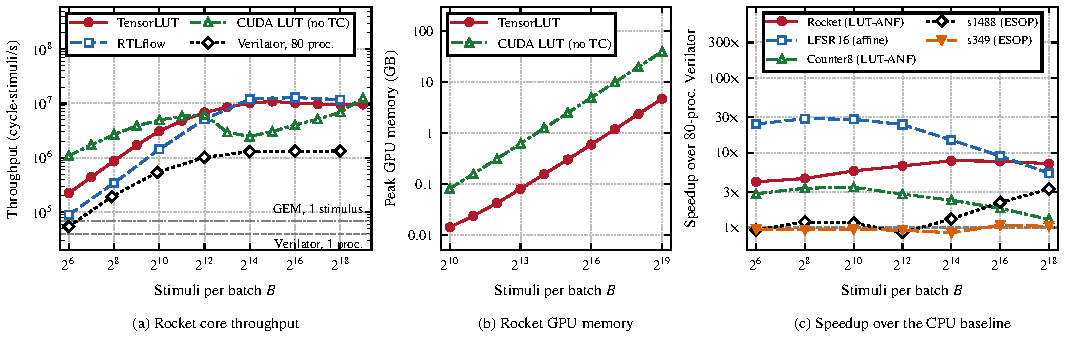
\includegraphics[width=\textwidth]{figs/batch_scaling.pdf}
\caption{Batch-size study. (a) Rocket-core throughput against batch size $B$ ($C=64$) for TensorLUT,
the CUDA-core LUT baseline, Verilator sharded over $\min(80,B)$ processes, and RTLflow; the dashed
line is one Verilator process and the dotted line is GEM simulating one stimulus. (b) Peak GPU memory of the two GPU simulators. (c) TensorLUT speedup over measured
80-process Verilator at the same $B$; the dashed line marks break-even. Curves are distinguished by
line style and marker as well as color.}
\Description{Three line charts. Panel a: Rocket throughput on a log scale. TensorLUT rises linearly
and flattens near ten million cycle-stimuli per second from two to the fourteenth stimuli on; the
CUDA-core baseline is faster below two to the twelfth, dips in the middle, and overtakes again at two
to the nineteenth; RTLflow is slower than TensorLUT up to two to the twelfth and about 1.2 times faster
above; 80-process Verilator flattens near 1.3 million; GEM's single-stimulus rate is a horizontal line
near seventy thousand. Panel b: GPU memory grows linearly
for both GPU simulators, with the CUDA-core baseline about eight times higher, reaching 39 GB. Panel c:
speedup over 80-process Verilator for five workloads; LFSR16 is highest, Rocket stays between four
and six times, Counter8 between one and three times, s1488 rises to three times at large batches,
and s349 stays at about one.}
\label{fig:batch}
\end{figure*}

\subsection{Methodology and Correctness}
\textbf{Platform.} All runs use one server. GPU results use one NVIDIA RTX~4090 (Ada, sm\_89,
24GB) with CUDA~13; the only exception is the CUDA-core baseline at $B=2^{19}$, which needs 39GB and
runs on a 48GB RTX~4090 board in the same machine. The CPU baseline runs on two Intel Xeon Gold 6148
sockets (2$\times$20 cores, 80 hardware threads, 2.4GHz) with 251GB of DRAM, using
Verilator~5.049~\cite{verilator} with \texttt{-O3} and GCC \texttt{-O3 -march=native}.

\textbf{Workloads.} We use three tiers. GF(2)-structured designs isolate the algebraic kernels.
ISCAS'89 sequential circuits~\cite{iscas89} (s27--s15850) exercise ESOP, LUT-ANF repair, and
differential checking. The large-RTL tier uses RTeAAL~Sim's generated RocketChip OctaCore
RTL~\cite{rteaal}: the full harness for Verilator/Dhrystone context, the Rocket DUT for Yosys
hierarchy scale, and the Rocket core with its submodules for TensorLUT lowering and throughput. The
golden reference is Icarus Verilog~\cite{icarus} on the original RTL.

\textbf{Measurement.} We report cycle$\cdot$stimuli/s. GPU runs replay a CUDA graph over
device-resident stimuli; generating the random stimuli on the GPU inside the timed loop leaves
Rocket throughput unchanged within measurement noise from $B=2^{10}$ to $2^{18}$. The CPU baseline gets the same
batch: we shard it over $P=\min(80,B)$ independent Verilator processes, each drawing its own random
inputs, and time from launch to the last exit. Both sides therefore pay their small-batch overheads.
For Rocket, Verilator simulates the same synthesized LUT/DFF netlist as TensorLUT, written back to
Verilog.

\textbf{Correctness.} The differential harness drives all PIs, holds reset for eight cycles on
ISCAS'89, and compares primary outputs at cycle boundaries. The regression suite covers the GF(2)
affine, whole-cone ANF, levelized LUT-ANF, and CUDA-graph replay paths, and checks ISCAS'89
primary-output traces against Icarus on s27, s349, s386, s510, s1488, and s5378. On the Rocket core,
the CPU netlist interpreter, the GPU gather backend, and TensorLUT agree on state and primary outputs
for $B=8$ over 256 cycles, and a $B=4096$, 256-cycle tensor-vs-gather run (1.05M
cycle$\cdot$stimuli) is also clean. The ESOP ablation is checked against a direct evaluator of the
synthesized AIG.

\subsection{How Large Must the Batch Be?}
Fig.~\ref{fig:batch} shows how large a batch TensorLUT needs, and for which batches and designs
it is slower than the baselines.

\textbf{Rocket.} TensorLUT throughput grows almost linearly with $B$ up to about $2^{12}$, the point
where tensor-core work starts to hide launch and synchronization latency. It reaches
$1.01\times10^7$ cycle$\cdot$stimuli/s at $B=2^{14}$, peaks at $1.09\times10^7$ at $2^{15}$, and stays
within 13\% of that peak up to $2^{19}$, so the large batches used elsewhere in this paper are not
required for peak throughput. Multi-process Verilator saturates at $1.33\times10^6$ once each of its
80 processes holds a few hundred seeds. TensorLUT is faster at every batch size we measured:
$4.1\times$ at $B=64$, $5.7\times$ at $2^{10}$, and $7.2$--$7.8\times$ from $2^{14}$ up.

At small batches the CUDA-core LUT baseline is faster than TensorLUT. Its per-thread lookup has a
lower fixed cost, and it leads up to $B=2^{11}$ ($4.9\times$ at $B=64$, $1.22\times$ at $2^{11}$).
Its throughput then drops to $2.5\times10^6$ at $2^{14}$ and rises again only gradually; TensorLUT
leads from $2^{12}$ to $2^{18}$, by $4.1\times$ at $2^{14}$ and $1.39\times$ at $2^{18}$. At
$2^{19}$ the CUDA-core baseline is $1.33\times$ faster ($12.7$ vs.\ $9.5\times10^6$), but it needs
39GB against TensorLUT's 4.7GB (Fig.~\ref{fig:batch}b). TensorLUT keeps stimuli and net values as
packed bits; from $2^{13}$ up its footprint is about $8\times$ smaller.

\textbf{Across designs.} Fig.~\ref{fig:batch}c repeats the comparison against measured 80-process
Verilator. The affine LFSR16 is 24--29$\times$ faster up to $B=2^{12}$ and falls to $5.3\times$ at
$2^{18}$ as Verilator amortizes process startup. Counter8 (LUT-ANF) stays between $1.3\times$ and
$3.5\times$. The two ESOP-compiled ISCAS circuits give the smallest gains. s1488 needs $2^{16}$ stimuli to
reach $2.2\times$ ($3.3\times$ at $2^{18}$). s349 stays at break-even ($0.85$--$1.07\times$): with 15
flip-flops and 137 ESOP cubes, one layer leaves most of each tensor tile empty, while a CPU core keeps
the whole circuit in its L1 cache. TensorLUT is faster than the CPU baseline when a regression
supplies at least a few thousand seeds and the design is large enough to fill tensor tiles. Rocket
satisfies both conditions; s349 satisfies only the first.

\subsection{Comparison with GPU Simulators}\label{sec:gpusim}
We ran two published GPU simulators on the same Rocket LUT/DFF netlist and the same RTX~4090.
RTLflow~\cite{rtlflow} transpiles Verilator's schedule to CUDA kernels that simulate one stimulus per
thread. GEM~\cite{gem} maps an and-inverter graph onto a virtual Boolean processor and simulates one
stimulus at a time; we re-synthesized the netlist to its cell library and checked the result
equivalent to the original. Both simulators match our reference on identical random stimuli: RTLflow
on all 9,496 output bits of 8 testbenches at cycles 16 and 64, and GEM on 72,499 output bits over 199
cycles. RTLflow inputs are drawn on the GPU, as for TensorLUT. Running RTLflow required four small
fixes, recorded in the artifact: a helper script missing from its repository, the target changed
from \texttt{sm\_80} to \texttt{sm\_89}, output-file splitting disabled to avoid an emitter crash, and
one misordered statement in its generated change-detection kernel. It builds with CUDA~12.4 and GCC~13;
GEM and TensorLUT use CUDA~13.

RTLflow is the stronger baseline (Fig.~\ref{fig:batch}a). TensorLUT is faster up to $2^{12}$ stimuli,
by $2.5\times$ at $B=64$, $2.2\times$ at $2^{10}$, and $1.33\times$ at $2^{12}$. From $2^{14}$ on,
RTLflow is $1.18$--$1.25\times$ faster ($1.28$ vs.\ $1.02\times10^7$ at $2^{16}$). RTLflow fixes the
batch size at compile time, and its Rocket build takes 9.7 minutes of transpilation and \texttt{nvcc}
compilation against 9.0s for TensorLUT (Fig.~\ref{fig:eval}c); its signal arrays take about 20KB per
seed against TensorLUT's 9KB. GEM serves a different use: it simulates one stimulus at
$6.9\times10^4$ cycles/s, $19\times$ TensorLUT's single-seed rate, and a second GEM instance on the
same GPU raises the aggregate by only $1.1\times$. TensorLUT's throughput passes GEM's between 16 and
32 stimuli. Against both, TensorLUT compiles fastest and leads at small and medium batches; at large
batches it reaches 80\% of RTLflow's throughput while every Boolean update runs as tensor-core
products.

\subsection{Compile Cost}
\begin{figure*}[t]
\centering
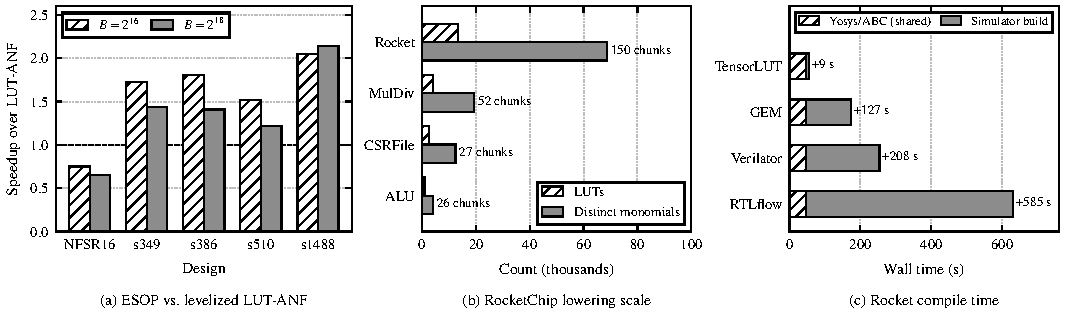
\includegraphics[width=\textwidth]{figs/eval_summary.pdf}
\caption{Compiler measurements. (a) ESOP synthesis speedup over per-layer LUT-ANF on the same netlist.
(b) RocketChip module scale after \texttt{abc -lut 6}; labels give tensor chunks at $\tau=512$.
(c) Rocket compile time: shared Yosys/ABC lowering (hatched) plus each simulator's own build.}
\Description{Three bar charts. Panel a: ESOP speedup over LUT-ANF at two batch sizes for five
designs; NFSR16 is below one, the ISCAS circuits are between 1.2 and 2.1. Panel b: LUT and monomial
counts for ALU, CSRFile, MulDiv and Rocket; Rocket has 13 thousand LUTs, 69 thousand monomials and
150 chunks. Panel c: compile time; all flows share 46 seconds of Yosys, then TensorLUT adds 9 seconds,
GEM 127, Verilator 208, and RTLflow 585 seconds.}
\label{fig:eval}
\end{figure*}

If the design changes between regressions, compile time is part of the cost. Fig.~\ref{fig:eval}c
splits the Rocket flow. Lowering the RTL to 6-LUTs with Yosys/ABC takes 46s and is shared by all
four simulators, which start from the same LUT/DFF netlist. TensorLUT then parses the netlist
(0.4s), levelizes it (0.06s), builds the ANF tensors (6.5s), and captures the CUDA graph for one
batch shape (2.0s): 9.0s in total. Verilator's C++ generation and \texttt{-O3} build take 208s,
GEM's AIG synthesis and mapping 127s, and RTLflow's transpilation and compilation 585s. Since
TensorLUT is also faster per cycle than Verilator at every batch size, it leads Verilator end to end
for any run length.
Only the graph capture depends on $B$. The ANF build is linear in the LUT count, because each LUT's
M\"obius transform costs at most $k\,2^k$ with $k\le6$; for much larger designs the monomial count
(Sec.~\ref{sec:mono}), not compile time, is the main cost.

\subsection{Large RTL and Throughput}
\textbf{Large RTL.} Table~\ref{tab:large} separates the full harness from the core-level plan;
\texttt{TestHarness} includes \texttt{SimAXIMem}, which accounts for its 2.15B memory bits. At
$B=2^{18}$, $C=64$, TensorLUT sustains $9.52\times10^6$ cycle$\cdot$stimuli/s on the Rocket core,
$242\times$ one Verilator process and $7.0\times$ an 80-process run. Capturing every primary output
in every cycle costs less than 1\% ($9.45\times10^6$). Normalized by circuit work, this point performs
$1.28\times10^{11}$ LUT evaluations/s, $6.53\times10^{11}$ monomial evaluations/s, and
$3.92\times10^{10}$ DFF updates/s, at about 9KiB of GPU memory per seed. For context, the full RTeAAL
8-core Dhrystone harness compiles to 98.3MB of C++ from 289 modules and runs at
$3.96\pm0.26$ kcycles/s in Verilator (three 550,352-cycle runs).

\begin{table}[tb]
\centering\footnotesize
\caption{RocketChip large-RTL measurements.}
\label{tab:large}
\setlength{\tabcolsep}{2.4pt}
\renewcommand{\arraystretch}{1.03}
\begin{tabular}{@{}p{.25\columnwidth}p{.67\columnwidth}@{}}
\toprule
Target & measurement\\
\midrule
OctaCore DUT & 168k cells; 5.26M wire bits; 1,088 memories; 2.25M mem bits\\
TestHarness & 169k cells; 5.29M wire bits; 1,164 memories; 2.15B mem bits\\
Rocket plan & 13.4k LUT; 4.1k DFF; 31 layers; 68.6k mono.; 150 chunks\\
Rocket check & $B=8,C=256$ CPU/gather/tensor: state/PO mismatches = 0\\
Verilator & same LUT/DFF netlist; 1 proc.: $3.94\times10^4$; 64 proc.: $1.29\times10^6$; 80 proc.: $1.35\times10^6$ cycle$\cdot$stimuli/s\\
CUDA no-TC & resident CUDA-graph LUT replay; $6.86\times10^6$ at $B=2^{18}$ (19.7GB); $1.27\times10^7$ at $B=2^{19}$ (39.5GB)\\
RTLflow & same netlist, one stimulus per thread; $1.17\times10^7$ at $B=2^{18}$; 9.7min build\\
GEM & same netlist as AIG cells; one stimulus; $6.9\times10^4$ cycles/s\\
TensorLUT & $9.52\times10^6$ at $B=2^{18}$ (2.35GB); $9.45\times10^6$ with PO capture; $9.53\times10^6$ at $B=2^{19}$ (4.69GB)\\
8-core harness & full Dhrystone in Verilator; 550k cycles; $3.96\pm0.26$ kcycles/s\\
\bottomrule
\end{tabular}
\end{table}

\textbf{Algebraic microbenchmarks.} At $B\ge2^{16}$, affine GF(2) designs reach $2.45$--$2.99\times10^9$
cycle$\cdot$stimuli/s, the fewest operations of any route. Nonlinear cones add monomial construction:
whole-cone ANF reaches $0.96$--$1.29\times10^9$, and levelized LUT-ANF reaches
$0.49$--$0.62\times10^9$ on Counter8. Against one Verilator process, LFSR16 is $285\times$ and Counter8
$57.5\times$ faster; Fig.~\ref{fig:batch}c gives the comparison against multi-process Verilator.

\subsection{LUT Width and Multiple GPUs}
\begin{table}[tb]
\centering\footnotesize
\caption{Rocket core under different LUT widths $k$ (\texttt{abc -lut $k$}), $B=2^{16}$, $C=64$, one
RTX~4090. Chunks use $\tau=512$.}
\label{tab:lutk}
\setlength{\tabcolsep}{0pt}
\begin{tabular*}{\columnwidth}{@{\extracolsep{\fill}}crrrrr@{}}
\toprule
$k$ & LUTs & layers & monomials & chunks & $10^6$ cycle$\cdot$stimuli/s\\
\midrule
4 & 18,325 & 49 & 61,724 & 149 & 8.09\\
5 & 15,658 & 37 & 63,036 & 142 & 9.61\\
6 & 13,406 & 31 & 68,606 & 150 & \textbf{10.19}\\
7 & 12,257 & 26 & 79,238 & 171 & 9.59\\
\bottomrule
\end{tabular*}
\end{table}

\textbf{LUT width.} The LUT mapper's $k$ sets a trade-off that a LUT-count objective does not see
(Table~\ref{tab:lutk}). Narrow LUTs give fewer monomials per LUT but deeper plans: $k=4$ needs 49
layers, and every layer adds two tensor-core stages, a synchronization, and net-state traffic. Wide
LUTs reduce the plan to 26 layers at $k=7$, but the monomial count grows to 79k because a $k$-input
LUT can carry up to $2^k$ terms. Throughput peaks at $k=6$, which is why we use \texttt{abc -lut 6}
throughout; a mapper that optimizes layers and monomials jointly is future work.

\textbf{Multiple GPUs.} Seeds are independent, so a batch shards across GPUs with no communication.
With $2^{16}$ seeds per RTX~4090 and stimuli drawn on each device, Rocket throughput goes from
$1.03\times10^7$ on one GPU to $2.04\times10^7$ on two ($1.98\times$) and $3.99\times10^7$ on four
($3.88\times$), $30\times$ the 80-process Verilator run. Four GPUs at only $2^{14}$ seeds each
still reach $3.96\times10^7$.

\subsection{Synthesis Ablations}\label{sec:mono}
\textbf{Tensor-core-aware synthesis.} Fig.~\ref{fig:eval}a compares ESOP with per-layer LUT-ANF on
the same synthesized netlist. ESOP maps each listed cone to one tensor-core layer and, after
passthrough stripping, usually needs far fewer monomials (s1488: $1457\to71$). On s1488 the speedup
grows from $2.05\times$ at $2^{16}$ to $2.14\times$ at $2^{18}$. s386 and s510 follow the same
pattern with smaller gains. NFSR16 is slower with ESOP: a shift register with one nonlinear
next-state bit and 15 copies has no depth to collapse, and ESOP only adds gather overhead.

\begin{table}[tb]
\centering\small
\caption{ISCAS'89 repair statistics (\texttt{abc -lut 6}); max is per-layer monomials, chk.\ uses
$\tau=512$.}
\label{tab:designs}
\setlength{\tabcolsep}{0pt}
\begin{tabular*}{\columnwidth}{@{\extracolsep{\fill}}lrrrrrr@{}}
\toprule
Design & DFFs & LUTs & lay. & mono. & max & chk.\\
\midrule
s27    & 3   & 5   & 2  & 40   & 34  & 2\\
s349   & 15  & 34  & 3  & 244  & 120 & 3\\
s641   & 17  & 68  & 5  & 343  & 93  & 5\\
s1423  & 74  & 158 & 11 & 992  & 226 & 11\\
s1488  & 6   & 167 & 4  & 1457 & 590 & 5\\
s5378  & 162 & 366 & 4  & 2359 & 734 & 7\\
s9234  & 135 & 311 & 5  & 1573 & 487 & 5\\
s13207 & 225 & 315 & 3  & 1770 & 909 & 5\\
s15850 & 157 & 215 & 4  & 1125 & 666 & 5\\
\bottomrule
\end{tabular*}
\end{table}

\textbf{Monomial growth.} A $k$-LUT can carry up to $2^k$ monomials, but the measured plans stay well
inside the tiled backend. On ISCAS'89 the largest per-layer count is 909 (s13207) and the largest
total is 2359 (s5378); $\tau=512$ needs at most seven chunks in Table~\ref{tab:designs}. Rocket is
the largest case: 68.6k distinct monomials over 31 layers, 8030 in the widest layer, and 150 tensor
chunks (Fig.~\ref{fig:eval}b). Where ESOP can collapse depth it cuts terms directly; elsewhere
TensorLUT uses more LUT-ANF chunks.

\section{Related Work}
\begin{table}[tb]
\centering\footnotesize
\caption{Scope of RTL simulation accelerators.}
\label{tab:prior}
\setlength{\tabcolsep}{2.6pt}
\renewcommand{\arraystretch}{1.08}
\begin{tabular}{@{}lllcc@{}}
\toprule
Work & Platform & Execution model & Batch & TC\\
\midrule
RTeAAL Sim~\cite{rteaal} & CPU & sparse tensor algebra & -- & --\\
GSIM~\cite{gsim} & CPU & generated simulator & -- & --\\
RepCut~\cite{repcut} & CPU & partitioned, multithreaded & -- & --\\
Manticore~\cite{manticore} & FPGA & 225-core BSP fabric & -- & --\\
Parendi~\cite{parendi} & IPU & 5888-core partitioning & -- & --\\
GEM~\cite{gem} & GPU & virtual VLIW on CUDA cores & -- & --\\
RTLflow~\cite{rtlflow} & GPU & Verilator$\to$CUDA kernels & \checkmark & --\\
TensorLUT & GPU & ANF$\to$b1 tensor-core GEMM & \checkmark & \checkmark\\
\bottomrule
\end{tabular}
\end{table}

Table~\ref{tab:prior} compares scope rather than speed; the systems were evaluated on different
designs and hardware. CPU simulators generate faster code from the RTL~\cite{rteaal,gsim} or
partition one instance across threads~\cite{repcut}; Manticore and Parendi spread one instance over
many small cores on an FPGA or an IPU~\cite{manticore,parendi}. On GPUs, GEM emulates an FPGA-like
Boolean processor for a single instance~\cite{gem}, and RTLflow transpiles Verilator's schedule to
CUDA kernels that run many stimuli at once~\cite{rtlflow}. RTLflow is the closest in workload;
Sec.~\ref{sec:gpusim} compares TensorLUT with both GPU simulators directly. TensorLUT differs in
where the Boolean update runs: on binary tensor cores, through an algebraic rewrite. Its low-bit MMA
machinery builds on tensor-core sparse kernels~\cite{tcgnn,dtcspmm,apntc,cutlass,ptx}, and its
Boolean form on ANF and Reed--Muller theory~\cite{reedmuller,wegener,bard,abc}.

\section{Scope and Extensions}\label{sec:scope}
TensorLUT is a throughput engine for regression batches. Its contract is 2-state, single-clock
LUT/DFF logic after frontend normalization. The features it lacks fall into two groups: those that
are engineering work within the same formulation, and those that conflict with it.

\textbf{Four-state values.} X and Z fit the formulation through a dual-rail encoding, with one bit for
the value and one for ``unknown.'' Each $k$-LUT becomes two Boolean functions of $2k$ inputs, its
output value and its output-unknown flag. Both are ordinary LUTs, so Eq.~\eqref{eq:anf} applies
unchanged. The cost is a higher degree bound: $2k=12$ instead of 6, and potentially many more monomials. Matching a
reference simulator bit for bit is a separate issue, because Verilog defines X-pessimism per operator,
not per LUT; the mapper would have to keep X-relevant operator boundaries.

\textbf{Multiple clocks.} Synchronous clocks with a known ratio need one plan per domain and a commit
schedule: at each global step only the domains that tick commit, which is a per-domain mask on the
existing commit gather. Asynchronous clocks need event ordering between domains. They do not fit a
cycle-batched model; we consider this a fundamental limit of the approach.

\textbf{Memories.} Large RAM and ROM are currently modeled in the harness, outside the tensor plan. A memory read is a
per-seed gather and a write is a scatter. Both run well on CUDA cores next to the tensor-core logic,
and the address streams of different seeds stay independent.

\textbf{Small batches and small designs.} This limit is inherent. Below about $2^{12}$ stimuli, or for
circuits as small as s349, the CUDA-core baseline or multi-process Verilator is as fast or faster
(Fig.~\ref{fig:batch}).

\textbf{Applications.} We measure simulation throughput, not a fuzzer or fault simulator built on it.
Fault simulation fits the same batch structure: one row per fault, with a stuck-at fault applied as a per-row mask on
a layer output. Building and validating that flow is our next step.

\textbf{Hardware.} The b1 MMA used here is exposed through warp-level \texttt{mma.sync} on recent
NVIDIA GPUs~\cite{ptx}. The counts in Eqs.~\eqref{eq:count} and~\eqref{eq:parity} can also be
computed exactly by INT8 MMA on $\{0,1\}$ operands, at eight times the operand footprint. At large batches RTLflow remains about $1.2\times$ faster
on Rocket. Ablating the layer kernel shows the time split across input gathering, the stage-1 degree
test, the stage-2 parity epilogue, and byte-granular net-state stores, not dominated by the MMAs. A
word-interleaved net-state layout and the 16-row \texttt{mma.m16n8k128} shape address the first and
last of these. Other planned work is a measured cost model for choosing $\tau$ and the ESOP route,
mapping objectives that reduce tensor padding, and fusion of adjacent small layers.

\section{Artifact}
Every number in this paper is produced by a script. The frontend drivers run Yosys and ABC and emit
the resource tables; the GPU and Verilator drivers log batch size, cycle count, backend, and workload
for each run; and the figure scripts emit the PDFs included here. A manifest records the checkout
commits, Yosys statistics, and workload arguments behind each table and figure. The code, benchmark
inputs, recorded measurements, and scripts are available at
\url{https://github.com/0xtaruhi/TensorLUT}.

\section{Conclusion}
TensorLUT runs a clock edge of a 2-state LUT/DFF netlist as two single-bit tensor-core products. The
first counts monomial supports and keeps those whose count equals their degree; the second combines
the surviving monomials and takes parity. A compiler routes each cone to an affine GF(2) GEMM, a
bounded ESOP layer, or levelized LUT-ANF chunks, and keeps the resulting tensors on the GPU. On one
RTX~4090 the Rocket core runs $7\times$ faster than 80 Verilator processes, beats the RTLflow GPU
simulator for batches up to $2^{12}$ seeds and reaches 80\% of its throughput above, compiles in 9s,
scales nearly linearly to four GPUs, and matches the reference traces bit for bit at every cycle
boundary.

% TODO(camera-ready): fill in funding sources, or delete this section.
\begin{acks}
This work was supported in part by [funding sources].
\end{acks}

\bibliographystyle{ACM-Reference-Format}
\bibliography{references}

\end{document}
